\documentclass[english]{tfgitic}
% per a fórmules químiques
\usepackage[version=4]{mhchem}
% Per dibuixar gràfics: base general i gràfics senzills
\usepackage{tikz}
\usetikzlibrary{arrows}
% Per dibuixar gràfics: circuits electrònics
\usepackage[europeanresistors,americaninductors]{circuitikz}
% Per dibuixar gràfics: diagrames diversos
\usepackage{pgfplots}
% Per escriure algoritmes
\usepackage[plain,figure]{algorithm2e}
% Per a usar taules elàstiques
\usepackage{tabularx}





% Indica quines bd bibliografiques usarem
\addbibresource{docum-tfe.bib}

% Marges en els algoritmes
\setlength{\algomargin}{4em}

% Versió de pgfplots a usar
\pgfplotsset{compat=newest}

\definecolor{tufte1}{rgb}{0.7,0.7,0.55}
\definecolor{yellowmarker}{HTML}{DEF440}

\pgfplotsset{

\end{enumerate}

\subsection*{Central Block}

\subsubsection*{Part I: Thesis Body}
Remember that «Parts» are only used if the manuscript contains
appendices. Otherwise, is better to avoid the «Part» subdivision.

\begin{enumerate}
\setcounter{enumi}{4}

\item \emph{Introduction} [Mandatory]\par
  This chapter introduces the thesis, including:
  \begin{itemize}
  \item The context, goals, and motivation of the project
  \item Summary of results
  \item Constraints (e.g., limited resources or budget)
  \item Specific objectives
  \item Outline of the document structure
  \end{itemize}

  It should also engage the reader’s interest and highlight the
  relevance of the work.

\item \emph{Background} [Mandatory]\par
  This chapter presents essential background knowledge:
  \begin{itemize}
  \item Prior work in the same field, including a critical and
    comparative review.
  \item Theoretical concepts, tools, languages, and methods used in
    the project.
  \end{itemize}

  This should be a concise overview, not a textbook. Relevant references
  should be provided.

\item \emph{Main Content} [Mandatory]\par
  This section consists of the main chapters describing the
  project. The structure depends on the specific nature of the work.

\item \emph{Economic Study} [Optional]\par
  If applicable, this chapter details economic considerations related
  to the project.

\item \emph{Environmental and Social Impact} [Optional]\par
  If applicable, this chapter addresses environmental and social
  aspects linked to the work.

\item \emph{Conclusions} [Mandatory]\par
  Summarizes the results, links them to the objectives, and discusses
  unmet goals and potential reasons.

\item \emph{Future Work} [Optional]\par
  Optionally, you may describe 2–4 relevant follow-up lines of work,
  briefly outlining how they could be approached.

\item \emph{Bibliography} [Mandatory]\par
  A non-numbered chapter listing all referenced works. It is
  automatically generated using the bibliography manager. See
  Chapter~\ref{cap:bibliografia} on page~\pageref{cap:bibliografia}.

\end{enumerate}

\subsubsection*{Part II: Appendices}

\begin{enumerate}
\setcounter{enumi}{12}

\item \emph{Appendices} [Optional]\par
  Appendices contain supporting material that is too detailed or
  extensive for the main text. Examples include:
  \begin{itemize}
  \item Data tables
  \item Maps or plans
  \item Survey forms
  \item Hard-to-access documents cited in the text
  \item Transcripts of interviews
  \item Source code
  \end{itemize}

  Whenever possible, cite such material rather than including it
  directly. If appendices are used, the document must be split into
  two parts: thesis body and appendices. If not, the \verb|\part{}|
  macros should be omitted.
\end{enumerate}





\printbibliography


\appendix

\part{Appendices}

\chapter{Best Practices for Writing a \acro{TFE} Manuscript}

\colorbox{yellow}{
  \begin{minipage}{1.0\linewidth}
    \Large\sffamily
    \begin{enumerate}

    \item Never manually force page breaks, adjust spacing
      arbitrarily, change fonts, or apply any other manual formatting
      tweaks. Let \LaTeX{} handle the layout, and focus your effort on
      the content.

    \item The text and its explanatory power are the core of your
      \acro{TFE} thesis. Your document is not a magazine, catalog, or
      promotional brochure.

    \item Figures should serve to clarify and support what is
      explained in the text. Including figures simply to «fill space»,
      to «make it look better», or because «there should be figures»
      is not acceptable. Include only those figures that are truly
      necessary, and design them with care. Ask yourself: if you
      removed a figure, would the explanation suffer? If not, the
      figure is probably unnecessary.

    \item Use floating figures, and do not force their placement. If
      the number of figures is appropriate, \LaTeX{}'s float mechanism
      will place them in optimal positions.

    \item Refer to all figures from the main text and explain them
      clearly to reinforce your intended message.

    \item Choose high-quality, academically sound bibliographic
      references. Avoid citing web pages from unreliable sources,
      commercial institutions, or general-interest content.

    \item Provide complete bibliographic entries. Include all
      available details about each source. Avoid submitting incomplete
      or vague references.

    \item In-text citations should support your argument, broaden the
      context, and clarify the authorship of ideas that are not your
      own.

    \end{enumerate}
    \smallskip
  \end{minipage}
}


\chapter{Version History of the \texttt{tfgitic} Class and Documentation}
\label{cap:historia}

\begin{tabularx}{\linewidth}{@{}lX@{}}
  \toprule
  \emph{Version} & \emph{Modifications} \\
  \midrule
  %current version
  8.2 & Some typos.\\
  8.1 & Add section numbers to pdf bookmarks.
  Improve some details in the manual.
  Solve typo contributed by Pau de las Heras.
  Small improvements to release script.
  More descriptive title for the manual.
  New macro \verb/\classversion/.\\

  8.0 & Class docum now in English, \fitx{docum-tfe-en}. New appendix
  about table typessetting.
  Upgrade and localise \texttt{siunitx} use.
  Improve the manuscript abstract.\\

  7.1 & Updated the minimum required versions for several packages.
  Improved internationalization (I18N).
  Added gender and number parameters to macros
  for defining people. Enhanced word hyphenation rules for Catalan.
  Introduced error messages for invalid metadata combinations.
  Typographic information is now reflected on the inside cover.
  Various corrections by Aleix Llusà. \\

  7.0 & Bug fixes contributed by Eric Roy.
  Updated to the latest version of the \texttt{sunitx} package.
  Added a section on figure and table captions.
  Introduced the «responsible statement» as required by anti-plagiarism
  regulations. Differentiated the roles of tutor and supervisor.
  Standardized project naming according to degree or master’s level.
  Replaced the \acro{tfg} acronym with the more general \acro{tfe}.
  Added option to indicate whether the \acro{tfe} is for a bachelor’s
  or a master’s program.
  Fixed an error in page numbering. \\

  6.5 & Improvements to the bibliography relay system. \\

  6.4 & Bug fixes. Updated the \acro{upc} logo in compliance with current regulations.
  Added documentation for the \texttt{C-c C-a} command in \texttt{AUCTeX}. Updated the
  \acro{cc} license to version 4.0. The \texttt{summary} and \texttt{abstract} environments
  now apply the correct orthotypography for each language and respect paragraph structure.
  Added a field for location (city) on the cover. Included additional comments on
  bibliography formatting. Deprecated the \texttt{summary} environment in favor
  of \texttt{abstract}. Updated bibliography. Generalized the class to support other
  degrees and schools. \\

  6.3 & Bug fixes. Major improvements to publishing tools. Modified and documented full
  magnitude notation. Fixed an error in the implementation of the \texttt{abstract}
  environment, which previously did not recognize paragraph breaks. \\

  6.2 & Minor improvements to documentation. \\

  6.1 & Removed minor warnings. Added version control to the \texttt{tfgitic} class. \\

  6.0 & Documentation now includes appendices on \LaTeX{} and \texttt{Emacs}. Added a
  chapter on writing mathematical expressions. Fixed the school name in the cover template. \\

  5.0 & Added support for both English and Catalan. Improved cover formatting. Added
  acknowledgments section. Expanded documentation. Introduced a new section on document
  structure. \\

  4.0 & Added automatic hyphenation and support for English quotation marks. \\

  3.0 & Bibliography is now included in the table of contents. \\

  2.0 & Added optional macro for defining subtitles. \\

  1.0 & Introduced the class history. Added commentary on line breaks in ligatures
  (such as the twin «l»). Added a new reference. Rewrote the section on appendices. \\

  \bottomrule
\end{tabularx}




\chapter{Very Brief Introduction to \LaTeX}
\label{ape:intro-latex}

\LaTeX{}~\cite{lamport94:_latex_ed} is a high-quality typesetting
system. It is not a \acro{wysiwyg} editor, but rather functions as a
compiler: you write your document in a «source language» and, after
compilation, obtain a file---typically in \texttt{pdf} format. \LaTeX{}
itself is that source language. It is a type of markup language: you
write the text and insert commands or «marks» that specify the
structure---for example, titles, lists, formulas, and so on.

The key benefit is this: when writing, you can focus entirely on
content, while the compiler handles formatting automatically. The
final layout depends on the document class being used. Changing the
class or its parameters results in a different appearance. This very
document, for example, uses a class that formats a thesis according to
the conventions for \acro{tfe} submissions.

A golden rule---the most important one---is: \emph{never override
  the formatting defined by the document class}. The appearance is the
exclusive responsibility of the class.

The source code of a \LaTeX{} document is written in a plain text file
using a text editor. For instance, in the file \fitx{document.tex},
the contents might look like this:

\begin{verbatim}
\documentclass[a4paper,12pt]{article}
\usepackage[catalan]{babel}

\title{Un exemple}
\author{Ramon Gener}

\begin{document}
\maketitle{}

\section{Introducció}
Això és un apartat d'exemple. I això que segueix una \emph{enumeració}:
\begin{enumerate}
\item Primer punt.
\item Segon punt.
\item Tercer punt.
\end{enumerate}
\end{document}
\end{verbatim}

To compile the document, run:
\begin{verbatim}
$ pdflatex document.tex
\end{verbatim}

After some messages appear in the terminal, the file
\fitx{document.pdf} will be generated.

Sometimes, a single compilation is not sufficient. To simplify the
process, you can use the command \ord|latexmk|, which automatically
runs the compiler as many times as needed. To install it:

\begin{verbatim}
$ sudo apt install latexmk
\end{verbatim}

This tool can also perform common tasks, such as generating a \acro{pdf} or
cleaning up auxiliary files. Refer to the \texttt{man} page for
details. To generate a \acro{pdf}:
\begin{verbatim}
$ latexmk -pdf document.tex
\end{verbatim}

If you're using the \texttt{emacs} editor---which we recommend---see
Appendix~\ref{ape:emacs}.

To learn the basics of \LaTeX{}, many resources are available. A
helpful and concise introduction is found
in~\cite{oetiker:_not_so_short_introd_latex}.



\chapter{Emacs Support}
\label{ape:emacs}

\texttt{Emacs}~\cite{foundation19:_gnu_emacs,stallman81:_emacs_exten_custom_self_displ_editor}
is the recommended text editor for working with \LaTeX{}. Support for
\LaTeX{} in \texttt{Emacs} is primarily provided through the extension
\texttt{AUCTeX}~\cite{thorup17:_auctex_sophis}, and secondarily via
the \texttt{RefTeX} extension~\cite{dominik09:_reftex_user_manual},
which works alongside AUCTeX to manage references and citations.

These tools offer powerful features, including:
\begin{itemize}
  \item Insertion of macros and environments via key commands.
  \item Automatic formatting of source code.
  \item Syntax highlighting for improved readability.
  \item Integration of the compile–preview workflow.
  \item Auto-completion of citations and references.
  \item Management of bibliography databases.
\end{itemize}

\section{Installation}

If needed, install the required packages via:
\begin{verbatim}
$ sudo apt-get install emacs
$ sudo apt-get install auctex
\end{verbatim}

Then, edit your \texttt{emacs} configuration file \fitx{~/.emacs},
adding the following lines to activate \texttt{RefTeX} when
\texttt{AUCTeX} is in use:
\begin{verbatim}
;; Enable RefTeX when AUCTeX is active
(add-hook 'LaTeX-mode-hook 'turn-on-reftex)
(setq reftex-plug-into-AUCTeX t)
\end{verbatim}

The next time you open \texttt{emacs}, the modes will be correctly
configured.

\section{Basic Usage}

When you open a file with the \fitx{.tex} extension, \texttt{emacs}
automatically enters «LaTeX mode». The menu bar will include:
\begin{itemize}
\item A «LaTeX» menu for inserting structures.
\item A «Command» menu for compiling and viewing the document.
\end{itemize}

Most commands are also available via keyboard shortcuts, which are
usually faster. Table~\ref{tab:ordres-emacs} lists some of the most
frequently used key bindings. Especially important is the \texttt{C-c
 C-c} command, which automatically determines and executes the next
appropriate compilation step.

\begin{table}
  \centering
  \begin{tabularx}{\linewidth}{@{}lX@{}}
    \toprule
    \emph{Shortcut} & \emph{Function} \\
    \midrule
    \texttt{C-c e} & Insert an environment; may prompt for parameters. \\
    \texttt{C-c C-s} & Insert a section, subsection, or chapter. \\
    \texttt{C-c RET} & Insert a macro, such as \texttt{author}. \\
    \texttt{Tab} & Insert a new item in a list environment (\texttt{itemize}, \texttt{enumerate}, \texttt{description}). \\
    \texttt{C-[} & Insert a citation, offering suggestions from the bibliography database. \\
    \texttt{C-c )} & Same as above---alternative citation shortcut. \\
    \texttt{C-c C-c} & Perform the next compilation step (e.g., compile or view, depending on context). \\
    \texttt{C-c a} & Compile and view the document in one step. If necessary, runs \texttt{biber} or other tools. Most commonly used command. \\
    \bottomrule
  \end{tabularx}
  \caption{Frequently used Emacs commands for working with \LaTeX{}. The prefix \texttt{C-} stands for the Control key.}
  \label{tab:ordres-emacs}
\end{table}

If you're editing a bibliography file with the \fitx{.bib} extension,
\texttt{Emacs} activates BibTeX/BibLaTeX mode, allowing for efficient
database management. You can insert entry templates (e.g.,
\texttt{@Book}), which include all fields---both mandatory and
optional (prefixed with \texttt{opt}). After filling in a field, press
\texttt{Tab} to jump to the next one. When done, the command
\texttt{C-c C-c} removes unused fields, checks for syntax errors, and
suggests a citation key. Just like that, your new reference is ready!



\chapter{How to Typeset Tables}
\label{ape:disseny-taules}

Poorly designed tables are a common flaw in \acro{tfe}
manuscripts. This appendix distills practical guidance from Bringhurst
and Tufte on how to design effective tables and shows how to implement
those ideas in \LaTeX{}.

It also presents real examples taken from theses: each original table
is analysed and then redesigned and typeset.

\section{Best Practices for Table Design}
\label{sec:good-pract-tables}

Bringhurst \cite[70]{bringhurst04:_elemen_typog_style} devotes several
pages to tabular typography. Püschel’s slides
\cite{püschel10:_small_guide_makin_nice_tables} offer a concise
\LaTeX{}-oriented summary. Designing tables is demanding; approach it
deliberately. Keep the following principles in mind:

\begin{enumerate}

\item \emph{Purpose and necessity}\par
  Use a table only when structure genuinely improves comprehension. If
  the information reads just as well linearly, prefer prose or a list.

  Every table must answer a clear question. Delete any column, row, or
  figure that does not contribute to that answer.

\item \emph{Economy and simplicity}\par
  Show the data, not the furniture. Minimise rules (lines), boxes,
  shading, and ornaments.

  Prefer white space over ruling. Spacing between columns or column
  groups normally replaces vertical rules entirely.

  Avoid «chartjunk»: gradients, heavy fills, gratuitous bold, repeated
  units in cells, and spurious decimals.

\item \emph{Hierarchy and emphasis}\par
  Build hierarchy with position, weight, and spacing---not
  decoration. The eye should locate the header first, then the logical
  groupings.

  Column headings may use a slightly different style (small caps,
  gentle letter-spacing, subtle weight change) but should not
  overpower the body.

  Totals or summary rows can be separated with a thin rule above,
  extra white space, or a modest typographic shift---reserve shouting
  (all caps, heavy bold) for real emergencies.

\item \emph{Rules (lines)}\par
  Use as few horizontal rules as possible: often just (a) a top rule,
  (b) a header/body separator, (c) an optional subtotal or total rule,
  and (d) a bottom rule.

  Avoid vertical rules; alignment and spacing should do the work.

  Keep strokes hairline to light. Thick rules dominate and break the
  rhythm of the page.

\item \emph{Alignment and numerals}\par
  Align numbers by meaning:
  \begin{itemize}
  \item Integers flush right.
  \item Decimals aligned on the separator (use the \texttt{S} column
    from \fitx{siunitx} or \fitx{dcolumn}).
  \item Put units in the header or a separate column---do not repeat a
    constant unit in every cell.
  \end{itemize}

  %Use tabular (lining) figures for numeric columns; proportional
  %figures are fine for prose.

  Use a true minus sign for negatives; reserve en-dashes for
  ranges. See point about dashes in Section~\ref{cap:ortotipografia}.

\item \emph{Consistency and precision}\par
  Round consistently. Do not imply precision the data do not have.

  Order rows and columns logically (chronology, magnitude,
  category). If the ordering principle is not obvious, state it.

\item \emph{Spacing and proportion}\par
  Row height: provide enough leading for legibility; avoid both
  «airless» stacking and gaping voids.

  Column separation: keep the smallest comfortable gap; a slightly
  wider gap can signal a group boundary.

  Keep tables within the main text measure unless a wider format is
  essential; very wide tables impede reading.

\item \emph{Typography inside cells}\par
  If the table is dense, set type slightly smaller than the running
  text (\qtyrange{0.5}{1}{pt}), but never so small that it strains the
  eye.

  Avoid competing emphases. Reserve bold or italics for one semantic
  layer, not both simultaneously.

  %Use small caps sparingly (e.g., for abbreviations in headers) to
  %keep texture calm.

\item \emph{Grouping and reading flow}\par
  Group related rows with white space, not thick rules. A small extra
  baseline skip (an «air line») is often enough.

  Left-align text columns; centre only very short, homogeneous labels.

  Avoid awkward wrapping of key identifiers. If a label is too long,
  abbreviate it and explain in a note.

\item \emph{Footnotes, sources, and notes}\par
  Annotate sparingly. Use superscript markers or symbols and collect
  explanations below the table in a smaller size.

  Captions should be concise and specific.

\item \emph{Accessibility and clarity}\par
  Do not rely on colour alone; differentiation must survive grayscale
  printing.

  Explain non-obvious abbreviations in the heading or a note.

  Ensure scanability: a reader should grasp what each column means and
  where totals lie within \qtyrange{2}{3}{\second}.

\item \emph{Avoid over-design}\par
  Resist boxing every cell. Grids imprison data; open layouts support comparison.

  Use shading only if hierarchy fails without it. If you must shade,
  keep it very light and consistent.

\end{enumerate}

\begin{table}
  \centering
  \begin{tabularx}{0.7\linewidth}{@{}lX@{}}
    \toprule
    \emph{Aspect} & \emph{Question} \\
    \midrule
    Necessity & Does a table genuinely improve clarity over prose? \\
    Hierarchy & Are headers / groups immediately identifiable? \\
    Lines & Have I removed every non-essential rule? \\
    Alignment & Are numerals and decimals properly aligned? \\
    Units & Are units placed in headers (not repeated)? \\
    Precision & Is decimal precision consistent and justified? \\
    Space & Is grouping conveyed by white space, not clutter? \\
    Caption & Is it concise, specific, and informative? \\
    Notes & Are footnotes / sources clear yet unobtrusive? \\
    Legibility & Is size/contrast acceptable in print? \\
    \bottomrule
  \end{tabularx}
  \caption{Good table checklist}
  \label{tab:table-checklist}
\end{table}

Table~\ref{tab:table-checklist} offers a brief checklist inspired by
the preceding principles. Use it to audit your tables.


\section{\LaTeX{} Implementation Hints}

\begin{itemize}
\item Load \texttt{booktabs}: \verb|\toprule|, \verb|\midrule|,
  \verb|\addlinespace|, \verb|\bottomrule|; avoid vertical rules.
\item Use \texttt{siunitx} \verb|S| columns for numeric alignment,
  rounding, and decimal alignment.
\item Put units in the column heading,
  e.g. \verb|\multicolumn{1}{c}{Voltage (\unit{\volt})}|.
\item Separate logical row groups with \verb|\addlinespace| rather
  than extra \verb|\midrule|s.
\item Keep captions succinct, e.g.\par
  \verb|\caption{Latency benchmarks for API endpoints ($n=500$).}|
\item Always proof a printout; adjust spacing and rule weight after
  seeing physical output.
\end{itemize}



\section{Table Examples}

\subsection*{Example 1}

\begin{figure}
  \centering
  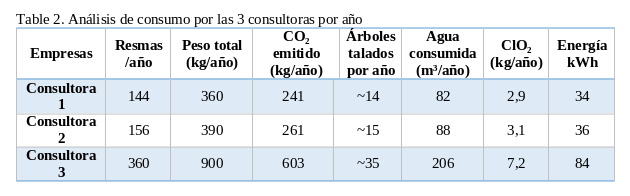
\includegraphics[width=0.9\linewidth]{taula-exemple-1.png}
  \caption{Original table for example 1}
  \label{fig:source-table-1}
\end{figure}

In this example we analyse the table in
Figure~\ref{fig:source-table-1}, taken from a master’s thesis. Several
issues contravene the best practices of
Section~\ref{sec:good-pract-tables}.
\begin{itemize}
\item Decoration (colour bands, etc.) carries no information and
  should be removed.
\item Bold is used even though it should be reserved for sectioning.
\item Centre alignment is poor for numeric columns.
\item Headings are verbose.
\item Columns could be hierarchised to aid reading.
\end{itemize}

\begin{table}
  \centering
  \sisetup{table-number-alignment = right}
  \begin{tabular}{
    l
    S[table-format=3]        % Resmas
    S[table-format=3]        % Peso total
    S[table-format=2]        % CO2 emitido
    S[table-format=3]        % Árboles (aprox, con ~)
    S[table-format=1.2]      % Agua consumida
    S[table-format=2]        % ClO2 (con decimal)
    S[table-format=3]        % Energía kWh
    }
    \toprule
    &
    \multicolumn{2}{c}{\emph{Papel consumido}}&
    \multicolumn{4}{c}{\emph{Consumo de recursos inducido}}&
    \multicolumn{1}{c}{\emph{Huella}}
    \\
    \cmidrule(rl){2-3} \cmidrule(rl){4-7} \cmidrule(lr){8-8}
    &
    {Resmas} &
    {Peso/\unit{\kilogram}} &
    {Árboles} &
    {Agua/\unit{\cubic\meter}} &
    {\ce{ClO2}/\unit{\kilogram}} &
    {Energía/\unit{\kWh}} &
    {\ce{CO2}/\unit{\kilogram}} \\
    \midrule
    1 & 144 & 360 & 14 &  82 & 2.9 & 34 & 241 \\
    2 & 156 & 390 & 15 &  88 & 3.1 & 36 & 261 \\
    3 & 360 & 900 & 35 & 206 & 7.2 & 84 & 603 \\
    \bottomrule
  \end{tabular}
    \caption{Redesign of table of Figure~\ref{fig:source-table-1}}
  \label{tab:redesigned-table-1}
\end{table}

The redesign in Table~\ref{tab:redesigned-table-1} addresses these
problems:
\begin{itemize}
\item All superfluous decoration is removed.
\item Non-essential rules\footnote{In typography, «rules» are
    horizontal or vertical lines.} are dropped: no vertical rules and
  only the necessary horizontals. The structure becomes clear through
  alignment and spacing.
\item Columns are aligned according to standard practice.
\item Columns are rearranged to allow meaningful grouping and a
  hierarchical header.
\item Repetitive temporal information («año») is moved to the caption.
\item Bold is avoided. The structure alone clarifies headers; only the
  top-level groups are emphasised to reveal hierarchy.
\item Company names were anonymised in the original; «Consultora 1»
  etc. adds width without meaning. Simple numbering suffices and
  shortens the table.
\end{itemize}
Headers are upright; their role is evident thanks to the horizontal
rules. Only the hierarchical layer is emphasised. In a simple,
non-hierarchical table, no emphasis would be needed. The result is
clearer and easier to read.

A good caption would be «Tabla 2: Consumo anual de papel de tres
consultoras, consumo inducido y impacto.»

Source code for the redesigned table:
\begin{verbatim}
\begin{table}
  \centering
  \sisetup{table-number-alignment = right}
  \begin{tabular}{
    l
    S[table-format=3]        % Resmas
    S[table-format=3]        % Peso total
    S[table-format=2]        % CO2 emitido
    S[table-format=3]        % Árboles (aprox, con ~)
    S[table-format=1.2]      % Agua consumida
    S[table-format=2]        % ClO2 (con decimal)
    S[table-format=3]        % Energía kWh
    }
    \toprule
    &
    \multicolumn{2}{c}{\emph{Papel consumido}}&
    \multicolumn{4}{c}{\emph{Consumo de recursos inducido}}&
    \multicolumn{1}{c}{\emph{Huella}}
    \\
    \cmidrule(rl){2-3} \cmidrule(rl){4-7} \cmidrule(lr){8-8}
    &
    {Resmas} &
    {Peso/\unit{\kilogram}} &
    {Árboles} &
    {Agua/\unit{\cubic\meter}} &
    {\ce{ClO2}/\unit{\kilogram}} &
    {Energía/\unit{\kWh}} &
    {\ce{CO2}/\unit{\kilogram}} \\
    \midrule
    1 & 144 & 360 & 14 &  82 & 2.9 & 34 & 241 \\
    2 & 156 & 390 & 15 &  88 & 3.1 & 36 & 261 \\
    3 & 360 & 900 & 35 & 206 & 7.2 & 84 & 603 \\
    \bottomrule
  \end{tabular}
  \caption{Consumo anual de papel de tres consultoras, consumo
    inducido y impacto.}
  \label{tab:redesigned-table-1}
\end{table}
\end{verbatim}



\subsection*{Example 2}

\begin{figure}
  \centering
  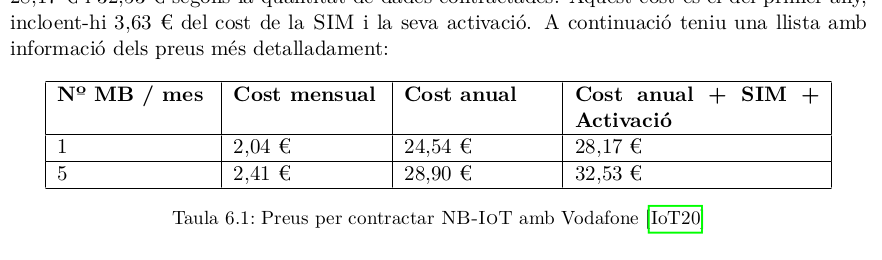
\includegraphics[width=0.9\linewidth]{taula-exemple-2.png}
  \caption{Original table for example 2}
  \label{fig:source-table-2}
\end{figure}

Figure~\ref{fig:source-table-2} shows another problematic table. This
one compares the cost of a couple of \acro{nb-iot} network connection
offers from the same company. These are the most salient issues:
\begin{itemize}
\item Excessive rules create a cage.
\item Columns are misaligned.
\item Units are repeated in every cell.
\item Bold headers look heavy.
\item Headings are too long, inflating column widths.
\item The table is forced inline instead of floating.
\item The distinction between SIM/setup costs and variable costs is
  unclear.
\end{itemize}

\begin{table}
  \centering
  % \sisetup{table-number-alignment = right}
  \begin{tabular}{
    S[table-format=1]        % MB
    S[table-format=1.2]        % Cost mensual
    S[table-format=2.2]        % Cost anual
    S[table-format=2.2]        % Cost total
    }
    \toprule
    &
    \multicolumn{2}{c}{\emph{Cost variable}}&
    \\
    \cmidrule(rl){2-3}
    {Velocitat} &
    {Mensual}&
    {Anual} &
    {Cost fix}
    \\
    {(\unit{\mega\byte\per\second})} &
    {(€)}&
    {(€)} &
    {(€)}
    \\
    \midrule
    1 & 2.04 & 24.54 & 3.63 \\
    5 & 2.41 & 28.9  & 3.63 \\
    \bottomrule
  \end{tabular}
  \caption{Redesign of table of Figure~\ref{fig:source-table-2}}
  \label{tab:redesigned-table-2}
\end{table}

The redesign appears in Table~\ref{tab:redesigned-table-2}. In the
redesign, the headings have been shortened and units are switen below
to keep good column spacing. The hierarchical relation in the header
is now explicit. A good caption would be «Taula 6.1: Preu del servei
\acro{nb-iot} de Vodafone, [IoT20]. El cost fix inclou la \acro{sim} i
la taxa de connexió.»

Its source is:
code is:
\begin{verbatim}
  \begin{tabular}{
    S[table-format=1]        % MB
    S[table-format=1.2]        % Cost mensual
    S[table-format=2.2]        % Cost anual
    S[table-format=2.2]        % Cost total
    }
    \toprule
    &
    \multicolumn{2}{c}{\emph{Cost variable}}&
    \\
    \cmidrule(rl){2-3}
    {Velocitat} &
    {Mensual}&
    {Anual} &
    {Cost fix}
    \\
    {(\unit{\mega\byte\per\second})} &
    {(€)}&
    {(€)} &
    {(€)}
    \\
    \midrule
    1 & 2.04 & 24.54 & 3.63 \\
    5 & 2.41 & 28.9  & 3.63 \\
    \bottomrule
  \end{tabular}
\end{verbatim}

\subsection*{Example 3}

\begin{figure}
  \centering
  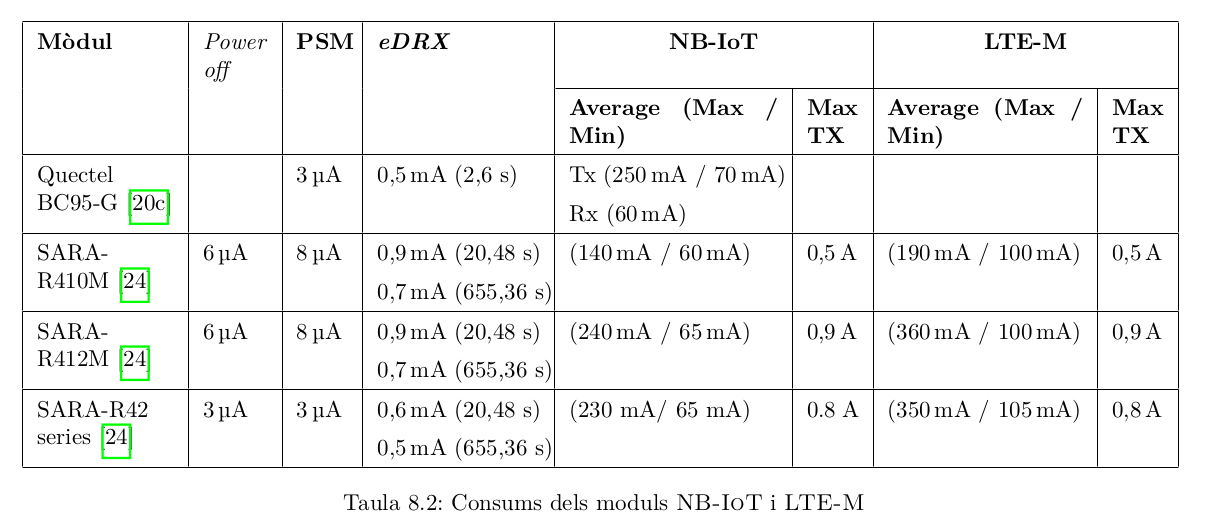
\includegraphics[width=0.9\linewidth]{taula-exemple-3.png}
  \caption{Original table for example 3}
  \label{fig:source-table-3}
\end{figure}

Figure~\ref{fig:source-table-3} compares several \acro{iot}
communication modules. Some support both \acro{nb-iot} and
\acro{lte-m}. Formal issues echo earlier examples:
\begin{itemize}
\item Too many rules.
\item Overly bold headers.
\item Units repeated in every entry.
\item Citations in the first column are likely repeated in the text
  and can be omitted.
\end{itemize}
Content-related problems are more serious:
\begin{itemize}
\item «dDRX» is opaque; some cells contain two values, themselves
  doubled.
\item «Average (max/min)» is ambiguous. Is it the average of
  maxima/minima or the extrema of averages?
\item The first row separates transmit and receive consumption; the
  others do not. What do their values represent?
\end{itemize}

\begin{table}
  \centering
  \newcommand{\na}{\textemdash}
  \begin{tabular}{
    l
    S[table-format=1.1]
    S[table-format=1.1]
    S[table-format=1.2]
    S[table-format=3.2]
    }
    \toprule
    & \multicolumn{2}{c}{\emph{Quiescent}}
    & \multicolumn{2}{c}{\emph{eDRX}}
    \\
    \cmidrule(lr){2-3} \cmidrule(lr){4-5}
    {Mòdul}
    & {Power off}
    & {PSM}
    & {Cycle}
    & {I\textsubscript{avg}}
    \\
    & {(\unit{\micro\ampere})}
    & {(\unit{\micro\ampere})}
    & {(\unit{\second})}
    & {(\unit{\milli\ampere})}
    \\
    \midrule
    Quectel BC95-G &   & 3 & 2.6    & 0.5 \\
    SARA-R410M     & 6 & 8 & 20.48  & 0.9 \\
                   &   &   & 655.36 & 0.7 \\
    SARA-R412M     & 6 & 8 & 20.48  & 0.9 \\
                   &   &   & 655.36 & 0.7 \\
    SARA-R42 series& 3 & 3 & 20.48  & 0.6 \\
                   &   &   & 655.36 & 0.5 \\
    \bottomrule
  \end{tabular}
  \caption{Redesign of table in Figure~\ref{fig:source-table-3}. Low
    power modes.}
  \label{tab:low-power}
\end{table}

\begin{table}
  \centering
  \begin{tabular}{@{}
    l
    S[table-format=2.0]
    S[table-format=3.0]
    S[table-format=1.1]
    S[table-format=3.0]
    S[table-format=3.0]
    S[table-format=1.1]
    @{}}
    \toprule
    &
    \multicolumn{3}{c}{\emph{NB-IoT}} &
    \multicolumn{3}{c}{\emph{LTE-M}}
    \\
    \cmidrule(r){2-4} \cmidrule(l){5-7}
    {Mòdul}
    & {$I_{avg}^{min}$}
    & {$I_{avg}^{max}$}
    & {Pic TX}
    & {$I_{avg}^{min}$}
    & {$I_{avg}^{max}$}
    & {Pic TX}
    \\
    & {(\unit{\milli\ampere})}
    & {(\unit{\milli\ampere})}
    & {(\unit{\ampere})}
    & {(\unit{\milli\ampere})}
    & {(\unit{\milli\ampere})}
    & {(\unit{\ampere})}
    \\
    \midrule
    Quectel BC95-G & 60 & 250 & { } & { } & { } & { } \\
    SARA-R410M     & 60 & 140 & 0.5 & 100 & 190 & 0.5 \\
    SARA-R412M     & 65 & 240 & 0.9 & 100 & 360 & 0.9 \\
    SARA-R42 series& 65 & 230 & 0.8 & 105 & 350 & 0.8 \\
    \bottomrule
  \end{tabular}
  \caption{Redesign of table in Figure~\ref{fig:source-table-3}. Tx/Rx power.}
  \label{tab:txrx-power}
\end{table}

Here the original is split into two complementary tables for clarity
and to avoid an unwieldy length. Table~\ref{tab:low-power} covers
consumption in low-power modes; Table~\ref{tab:txrx-power} focuses on
transmit/receive power. The source code for both tables follows:
\begin{verbatim}
  \begin{tabular}{
    l
    S[table-format=1.1]
    S[table-format=1.1]
    S[table-format=1.2]
    S[table-format=3.2]
    }
    \toprule
    & \multicolumn{2}{c}{\emph{Quiescent}}
    & \multicolumn{2}{c}{\emph{eDRX}}
    \\
    \cmidrule(lr){2-3} \cmidrule(lr){4-5}
    {Mòdul}
    & {Power off}
    & {PSM}
    & {Cycle}
    & {I\textsubscript{avg}}
    \\
    & {(\unit{\micro\ampere})}
    & {(\unit{\micro\ampere})}
    & {(\unit{\second})}
    & {(\unit{\milli\ampere})}
    \\
    \midrule
    Quectel BC95-G &   & 3 & 2.6    & 0.5 \\
    SARA-R410M     & 6 & 8 & 20.48  & 0.9 \\
                   &   &   & 655.36 & 0.7 \\
    SARA-R412M     & 6 & 8 & 20.48  & 0.9 \\
                   &   &   & 655.36 & 0.7 \\
    SARA-R42 series& 3 & 3 & 20.48  & 0.6 \\
                   &   &   & 655.36 & 0.5 \\
    \bottomrule
  \end{tabular}
\end{verbatim}

\begin{verbatim}
  \begin{tabular}{@{}
    l
    S[table-format=2.0]
    S[table-format=3.0]
    S[table-format=1.1]
    S[table-format=3.0]
    S[table-format=3.0]
    S[table-format=1.1]
    @{}}
    \toprule
    &
    \multicolumn{3}{c}{\emph{NB-IoT}} &
    \multicolumn{3}{c}{\emph{LTE-M}}
    \\
    \cmidrule(r){2-4} \cmidrule(l){5-7}
    {Mòdul}
    & {$I_{avg}^{min}$}
    & {$I_{avg}^{max}$}
    & {Pic TX}
    & {$I_{avg}^{min}$}
    & {$I_{avg}^{max}$}
    & {Pic TX}
    \\
    & {(\unit{\milli\ampere})}
    & {(\unit{\milli\ampere})}
    & {(\unit{\ampere})}
    & {(\unit{\milli\ampere})}
    & {(\unit{\milli\ampere})}
    & {(\unit{\ampere})}
    \\
    \midrule
    Quectel BC95-G & 60 & 250 & { } & { } & { } & { } \\
    SARA-R410M     & 60 & 140 & 0.5 & 100 & 190 & 0.5 \\
    SARA-R412M     & 65 & 240 & 0.9 & 100 & 360 & 0.9 \\
    SARA-R42 series& 65 & 230 & 0.8 & 105 & 350 & 0.8 \\
    \bottomrule
  \end{tabular}
\end{verbatim}

\subsection*{Example 4}

\begin{figure}[tb]
  \centering
  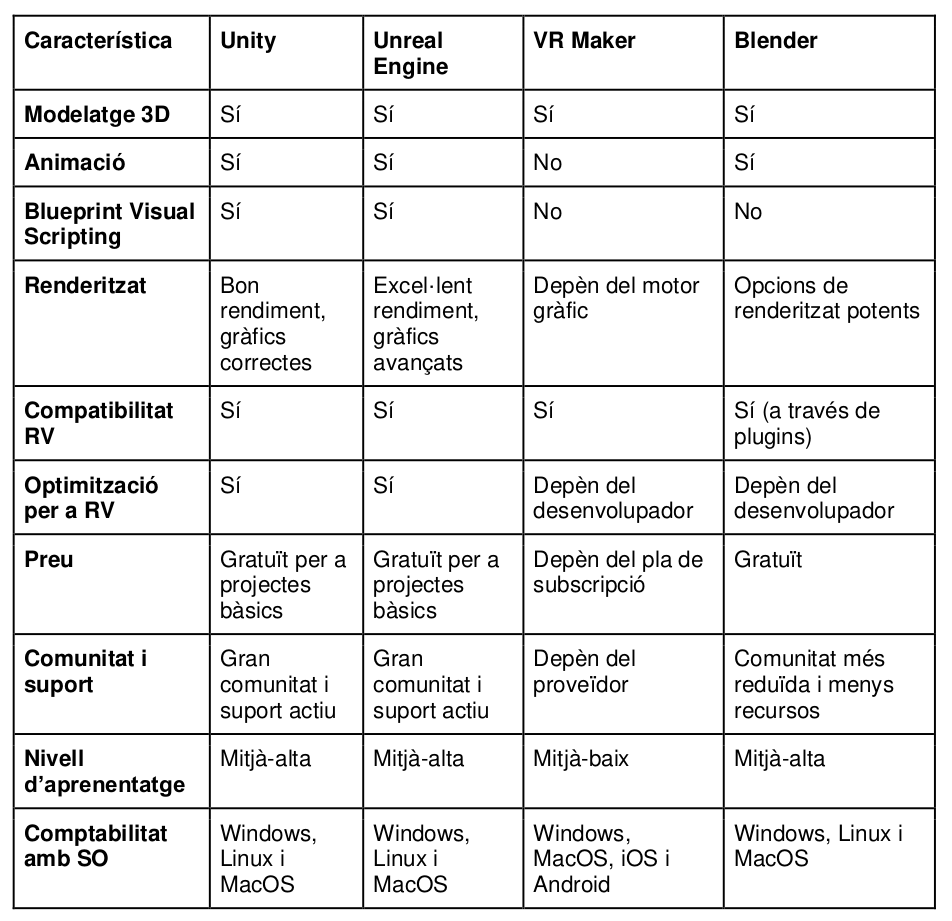
\includegraphics[width=0.7\linewidth]{taula-exemple-4.png}
  \caption{Original table for example 4}
  \label{fig:source-table-4}
\end{figure}

The table in Figure~\ref{fig:source-table-4} illustrates a non-numeric
comparison (virtual-reality software). Its flaws are familiar:
\begin{itemize}
\item Again, an abusive use of rules—very common!
\item Bold is used even though sectioning already claims it.
\item Several cells are too verbose.
\end{itemize}

\begin{table}[tb]
  \centering
  \small
  \newcolumntype{L}{>{\raggedright\arraybackslash}X}
  \renewcommand{\arraystretch}{1.05}
  \newcommand{\Lone}[1]{\emph{#1}}              % top level
  \newcommand{\Ltwo}[1]{\hspace{1.25em}#1}       % 2nd level

  \begin{tabularx}{0.95\linewidth}{@{} l L L L L @{}}
    \toprule
    Característica & Unity & Unreal Engine & VR Maker & Blender \\
    \midrule

    \Lone{Funcionalitat bàsica} \\
    \Ltwo{Modelatge 3D}              & Sí & Sí & Sí & Sí \\
    \Ltwo{Animació}                  & Sí & Sí & No & Sí \\
    \Ltwo{Visual scripting}          & Sí & Sí & No & No \\
    \addlinespace[0.6ex]

    \Lone{Rendiment} \\
    \Ltwo{Renderitzat}               & Bon rendiment; gràfics correctes
                                     & Exce\l.lent; gràfics avançats
                                     & Depèn del motor
                                     & Moltes opcions de render \\
    \Ltwo{Optimització RV}           & Sí & Sí & Depèn del dev & Depèn del dev \\
    \addlinespace[0.6ex]

    \Lone{Compatibilitat} \\
    \Ltwo{Amb  RV}                   & Sí & Sí & Sí & Sí (plugins) \\
    \Ltwo{S. Operatiu}               & Win, Linux, macOS
                                     & Win, Linux, macOS
                                     & Win, macOS, iOS, Android
                                     & Win, Linux, macOS \\
    \addlinespace[0.6ex]

    \Lone{Cost i suport} \\
    \Ltwo{Preu}                      & Gratuït bàsic & Gratuït bàsic & Segons subscripció & Gratuït \\
    \Ltwo{Comunitat}                 & Molt activa
                                     & Molt activa
                                     & Segons proveïdor
                                     & Més petita / menys recursos \\
    \Ltwo{Nivell aprenentatge}       & Mitjà-alt & Mitjà-alt & Mitjà-baix & Mitjà-alt \\
    \bottomrule
  \end{tabularx}
  \caption{Redesign of table shown in Figure~\ref{fig:source-table-4}}
  \label{tab:soft-comparison}
\end{table}

Table~\ref{tab:soft-comparison} presents the redesign. Improvements
include:
\begin{itemize}
\item Removal of unnecessary rules.
\item Reduction and normalisation of emphasis.
\item Shortened cell contents.
\item Rows reordered for a more meaningful sequence.
\item Added vertical hierarchy for easier scanning.
\item Slightly reduced type size to save space.
\end{itemize}

The source code is:
\begin{verbatim}
  \newcolumntype{L}{>{\raggedright\arraybackslash}X}
  \renewcommand{\arraystretch}{1.05}
  \newcommand{\Lone}[1]{\emph{#1}}              % top level
  \newcommand{\Ltwo}[1]{\hspace{1.25em}#1}       % 2nd level

  \begin{tabularx}{0.95\linewidth}{@{} l L L L L @{}}
    \toprule
    Característica & Unity & Unreal Engine & VR Maker & Blender \\
    \midrule

    \Lone{Funcionalitat bàsica} \\
    \Ltwo{Modelatge 3D}              & Sí & Sí & Sí & Sí \\
    \Ltwo{Animació}                  & Sí & Sí & No & Sí \\
    \Ltwo{Visual scripting}          & Sí & Sí & No & No \\
    \addlinespace[0.6ex]

    \Lone{Rendiment} \\
    \Ltwo{Renderitzat}               & Bon rendiment; gràfics correctes
                                     & Exce\l.lent; gràfics avançats
                                     & Depèn del motor
                                     & Moltes opcions de render \\
    \Ltwo{Optimització RV}           & Sí & Sí & Depèn del dev & Depèn del dev \\
    \addlinespace[0.6ex]

    \Lone{Compatibilitat} \\
    \Ltwo{Amb  RV}                   & Sí & Sí & Sí & Sí (plugins) \\
    \Ltwo{S. Operatiu}               & Win, Linux, macOS
                                     & Win, Linux, macOS
                                     & Win, macOS, iOS, Android
                                     & Win, Linux, macOS \\
    \addlinespace[0.6ex]

    \Lone{Cost i suport} \\
    \Ltwo{Preu}                      & Gratuït bàsic & Gratuït bàsic &
                                       Segons subscripció & Gratuït \\
    \Ltwo{Comunitat}                 & Molt activa
                                     & Molt activa
                                     & Segons proveïdor
                                     & Més petita / menys recursos \\
    \Ltwo{Nivell aprenentatge}       & Mitjà-alt & Mitjà-alt & Mitjà-baix &
                                     Mitjà-alt \\
    \bottomrule
  \end{tabularx}
\end{verbatim}



\end{document}

%%% Local Variables:
%%% mode: latex
%%% TeX-master: t
%%% LaTeX-biblatex-use-Biber: t
%%% End:
